\tikzset{every picture/.style={line width=0.75pt}} %set default line width to 0.75pt        

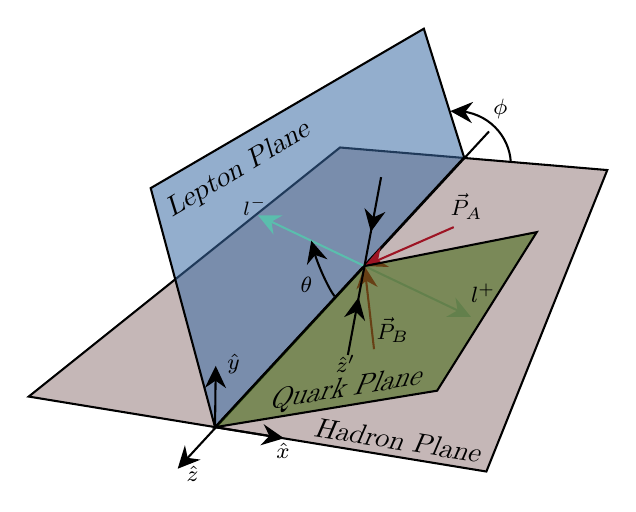
\begin{tikzpicture}[x=0.75pt,y=0.75pt,yscale=-1,xscale=1]
%uncomment if require: \path (0,300); %set diagram left start at 0, and has height of 300

%Straight Lines [id:da9360270151188433] 
\draw [color={rgb, 255:red, 90; green, 190; blue, 173 }  ,draw opacity=1 ]   (380.55,150.49) -- (332,127.36) ;
\draw [shift={(383.26,151.78)}, rotate = 205.47] [fill={rgb, 255:red, 90; green, 190; blue, 173 }  ,fill opacity=1 ][line width=0.08]  [draw opacity=0] (10.72,-5.15) -- (0,0) -- (10.72,5.15) -- (7.12,0) -- cycle    ;
%Shape: Polygon [id:ds3246920650393613] 
\draw  [fill={rgb, 255:red, 173; green, 152; blue, 152 }  ,fill opacity=0.7 ] (448.98,81.1) -- (390.73,226.35) -- (170.23,190.23) -- (238.46,135.64) -- (320.22,70.23) -- cycle ;
%Shape: Polygon [id:ds8122410861225874] 
\draw  [color={rgb, 255:red, 0; green, 0; blue, 0 }  ,draw opacity=1 ][fill={rgb, 255:red, 59; green, 107; blue, 164 }  ,fill opacity=0.55 ] (360.6,13) -- (229,89.8) -- (260,205) -- (380,75) -- cycle ;
%Straight Lines [id:da1607044272265945] 
\draw    (392,62.5) -- (244.03,222.8) ;
\draw [shift={(242,225)}, rotate = 312.71] [fill={rgb, 255:red, 0; green, 0; blue, 0 }  ][line width=0.08]  [draw opacity=0] (10.72,-5.15) -- (0,0) -- (10.72,5.15) -- (7.12,0) -- cycle    ;
%Straight Lines [id:da192804704893637] 
\draw [color={rgb, 255:red, 157; green, 20; blue, 36 }  ,draw opacity=1 ]   (375,108.6) -- (334.75,126.16) ;
\draw [shift={(332,127.36)}, rotate = 336.43] [fill={rgb, 255:red, 157; green, 20; blue, 36 }  ,fill opacity=1 ][line width=0.08]  [draw opacity=0] (10.72,-5.15) -- (0,0) -- (10.72,5.15) -- (7.12,0) -- cycle    ;
%Straight Lines [id:da9707379686817308] 
\draw [color={rgb, 255:red, 157; green, 20; blue, 36 }  ,draw opacity=1 ]   (336.6,167.4) -- (332.34,130.34) ;
\draw [shift={(332,127.36)}, rotate = 83.45] [fill={rgb, 255:red, 157; green, 20; blue, 36 }  ,fill opacity=1 ][line width=0.08]  [draw opacity=0] (10.72,-5.15) -- (0,0) -- (10.72,5.15) -- (7.12,0) -- cycle    ;
%Straight Lines [id:da6271845903433381] 
\draw [color={rgb, 255:red, 90; green, 190; blue, 173 }  ,draw opacity=1 ]   (332,127.36) -- (283.45,104.23) ;
\draw [shift={(280.74,102.94)}, rotate = 25.47] [fill={rgb, 255:red, 90; green, 190; blue, 173 }  ,fill opacity=1 ][line width=0.08]  [draw opacity=0] (10.72,-5.15) -- (0,0) -- (10.72,5.15) -- (7.12,0) -- cycle    ;
%Curve Lines [id:da8650973959260518] 
\draw    (317.57,141.86) .. controls (315.24,139.01) and (309.36,127.16) .. (306.99,117.95) ;
\draw [shift={(306.37,115.15)}, rotate = 74.54] [fill={rgb, 255:red, 0; green, 0; blue, 0 }  ][line width=0.08]  [draw opacity=0] (10.72,-5.15) -- (0,0) -- (10.72,5.15) -- (7.12,0) -- cycle    ;
%Straight Lines [id:da8376735939956365] 
\draw    (260,205) -- (290.26,209.86) ;
\draw [shift={(293.22,210.33)}, rotate = 189.12] [fill={rgb, 255:red, 0; green, 0; blue, 0 }  ][line width=0.08]  [draw opacity=0] (10.72,-5.15) -- (0,0) -- (10.72,5.15) -- (7.12,0) -- cycle    ;
%Straight Lines [id:da23422313993045396] 
\draw    (260,205) -- (260.3,178.44) ;
\draw [shift={(260.33,175.44)}, rotate = 90.65] [fill={rgb, 255:red, 0; green, 0; blue, 0 }  ][line width=0.08]  [draw opacity=0] (10.72,-5.15) -- (0,0) -- (10.72,5.15) -- (7.12,0) -- cycle    ;
%Straight Lines [id:da6033196978161374] 
\draw    (340,84.52) -- (332,127.36) ;
\draw [shift={(335.08,110.86)}, rotate = 280.58] [fill={rgb, 255:red, 0; green, 0; blue, 0 }  ][line width=0.08]  [draw opacity=0] (10.72,-5.15) -- (0,0) -- (10.72,5.15) -- (7.12,0) -- cycle    ;
%Shape: Polygon [id:ds8570377916667694] 
\draw  [fill={rgb, 255:red, 60; green, 101; blue, 10 }  ,fill opacity=0.55 ] (415,111) -- (367,187.4) -- (260,205) -- (332,127.36) -- cycle ;
%Straight Lines [id:da24422947787646188] 
\draw    (332,127.36) -- (324,170.19) ;
\draw [shift={(329.19,142.38)}, rotate = 100.58] [fill={rgb, 255:red, 0; green, 0; blue, 0 }  ][line width=0.08]  [draw opacity=0] (10.72,-5.15) -- (0,0) -- (10.72,5.15) -- (7.12,0) -- cycle    ;
%Curve Lines [id:da6714496890784999] 
\draw [color={rgb, 255:red, 0; green, 0; blue, 0 }  ,draw opacity=1 ]   (402.47,77.08) .. controls (401.8,65) and (391.79,52.99) .. (376.17,52.63) ;
\draw [shift={(373.38,52.69)}, rotate = 3.59] [fill={rgb, 255:red, 0; green, 0; blue, 0 }  ,fill opacity=1 ][line width=0.08]  [draw opacity=0] (10.72,-5.15) -- (0,0) -- (10.72,5.15) -- (7.12,0) -- cycle    ;

% Text Node
\draw (392.6,45.56) node [anchor=north west][inner sep=0.75pt]  [font=\fontsize{0.82em}{0.99em}\selectfont]  {$\phi $};
% Text Node
\draw (299.71,131.28) node [anchor=north west][inner sep=0.75pt]  [font=\fontsize{0.82em}{0.99em}\selectfont]  {$\theta $};
% Text Node
\draw (272.09,92.84) node [anchor=north west][inner sep=0.75pt]  [font=\fontsize{0.71em}{0.85em}\selectfont]  {$l^{-}$};
% Text Node
\draw (381.89,134.34) node [anchor=north west][inner sep=0.75pt]  [font=\fontsize{0.82em}{0.99em}\selectfont]  {$l^{+}$};
% Text Node
\draw (288.09,211.04) node [anchor=north west][inner sep=0.75pt]  [font=\fontsize{0.82em}{0.99em}\selectfont]  {$\hat{x}$};
% Text Node
\draw (244.76,222.38) node [anchor=north west][inner sep=0.75pt]  [font=\fontsize{0.82em}{0.99em}\selectfont]  {$\hat{z}$};
% Text Node
\draw (264.42,168.49) node [anchor=north west][inner sep=0.75pt]  [font=\fontsize{0.82em}{0.99em}\selectfont]  {$\hat{y}$};
% Text Node
\draw (234.68,94.28) node [anchor=north west][inner sep=0.75pt]  [font=\normalsize,rotate=-329.15,xslant=0.24] [align=left] {Lepton Plane};
% Text Node
\draw (289.02,184.79) node [anchor=north west][inner sep=0.75pt]  [font=\normalsize,rotate=-350.75,xslant=0.62] [align=left] {Quark Plane};
% Text Node
\draw (310.13,198.85) node [anchor=north west][inner sep=0.75pt]  [font=\normalsize,rotate=-9.21,xslant=0.25] [align=left] {Hadron Plane};
% Text Node
\draw (316.76,168.73) node [anchor=north west][inner sep=0.75pt]  [font=\fontsize{0.82em}{0.99em}\selectfont]  {$\hat{z} '$};
% Text Node
\draw (372.05,91.11) node [anchor=north west][inner sep=0.75pt]  [font=\fontsize{0.82em}{0.99em}\selectfont]  {$\vec{P}_{A}$};
% Text Node
\draw (336.3,150.78) node [anchor=north west][inner sep=0.75pt]  [font=\fontsize{0.82em}{0.99em}\selectfont]  {$\vec{P}_{B}$};


\end{tikzpicture}

